% !TEX root =../thesis-letomes.tex

\chapter{Introduction}
Colonization and proliferation has long been an ambition for humanity. With the earth fully explored (more or less), the next obvious frontier is space. Particularly our moon, and the relatively close and temperate Mars. In a lunar or Martian colony scenario, the first several decades will certainly be completely reliant on continuous support from earth, ferrying supplies and humans between the bodies. However, transporting mass into space is very costly. In a presentation given in 2005, the then NASA Administrator Michael Griffin mentioned the cost of launching payload into LEO was estimated to be $\$10,000$/kg \cite[p.~344]{Rapp2016}. Since then private space enterprise have pushed down the prices much further. The SpaceX Falcon Heavy launch vehicle had it's maiden launch on February 6, 2018, and can launch a payload of \SI{63800}{\kg} into LEO at a cost of $\$90$ million, equivalent to $\$710$/kg \cite{SpaceX}.

The Trump administration have pledged to sending astronauts back around the Moon in 2023, and land astronauts on the surface no later than the late 2020s, and have a long-term presence on the Moon \cite{NASA2018}, even mentioning using water on the surface as rocket fuel for Mars and beyond. NASA also plans to have boots on Mars in 2033 \cite{Mack}.

SpaceX maintains an aspirational goal of sending first cargo to Mars in 2022, and both cargo and human crew to Mars in 2024 \cite{SpaceXa}, with Elon Musk suggesting initiating base building on Mars as early as 2028 \cite{Williams}. The earliest tests of the BFR (Big Falcon Rocket \footnote{Unofficially the F is also known for a more colorful adjective}) is expected in 2019 \cite{SpaceXa}, see \cref{fig:musk-launch-vehicles} for launch vehicle overview.

\begin{figure}[ht]
	\centering
	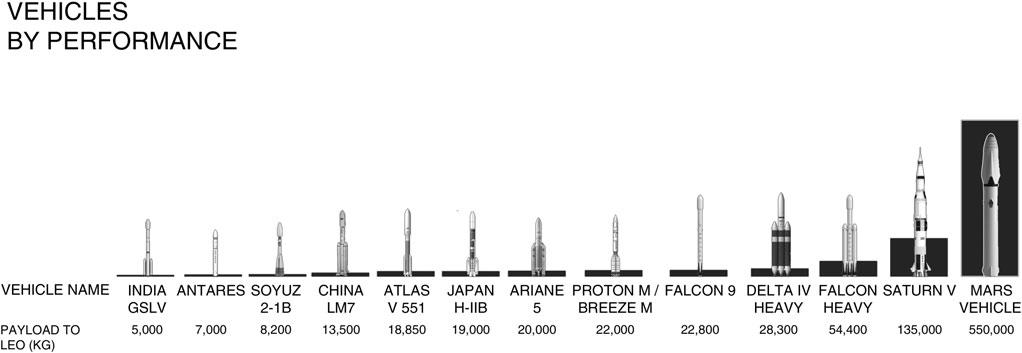
\includegraphics[width=0.90\linewidth]{fig/musk-launch-vehicles.jpg}
	\caption{Current and historic launch vehicles by performance (payload capacity) and relative size. The Mars Vehicle by SpaceX will have roughly 4 times the performance of Saturn V (Image: \cite{Musk}.}
	\label{fig:musk-launch-vehicles}
\end{figure}

SpaceX was founded in 2002 to revolutionize space technology, with the ultimate goal of enabling people to live on other planets \cite{SpaceXb}. SpaceX founder Elon Musk estimates that the threshold for a self-sustaining population on Mars is a million people \cite{Musk}. Musk reckons this will be done on the order of 10,000 trips with 100 people per ship, with up to 200 people later to reduce cost per person. Furthermore he notes:

\begin{displayquote}
But you would also need a lot of cargo to support those people. In fact, your cargo to person ratio is going to be quite high. It would probably be 10 cargo trips for every human trip, so more like 100,000 trips. And we’re talking 100,000 trips of a giant spaceship.
\end{displayquote}

The classic trajectory from Earth to Mars is the Hohmann transfer orbit, one half on an elliptical orbit around the Sun, that has a trip time of roughly 260 days or 8.5 months, as demonstrated in \cref{apx:mars-hohmann-derivations}. This assumes minimum delta-v scenario where one wants the cheapest way to Mars in delta-v (delta-v is the change in velocity which is a vehicle independent ``cost'' of maneuvers, proportional to fuel expenditure requirements for specific vehicles). For the trips carrying humans onboard, Musk is planning on trip times between 90 and 150 days for the next 20 years, even speculating as low as 30 days in the more distant future \cite{Musk}, see \cref{fig:musk-trip-time}.

\begin{figure}[ht]
	\centering
	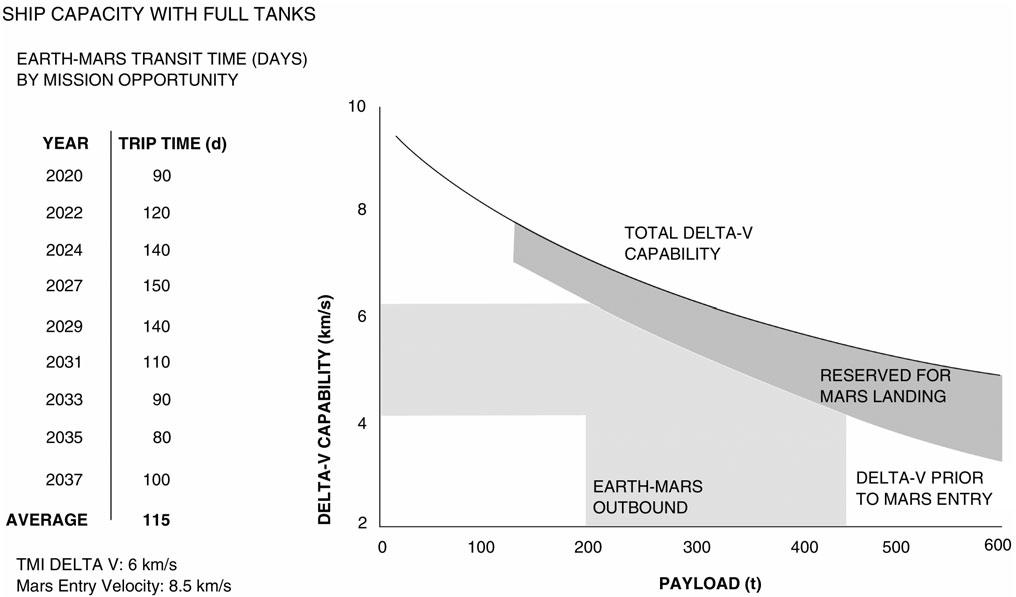
\includegraphics[width=1.0\linewidth]{fig/musk-trip-time.jpg}
	\caption{SpaceX estimated schedule for Earth-Mars transit time (in days). The trip time is increasing in the first decade, likely due to increasing the people capacity from 100 towards 200 people, going down again due to increases in vehicle performance, with Musk speculating it will eventually reach 30 days. Earth and Mars aligns every 26 months, which is why we see launch windows roughly 2 years apart.}
	\label{fig:musk-trip-time}
\end{figure}

We will now shift our attention back to the point about 9/10 of the 100,000 trips are going to be carrying materials instead of people. In 2000 \cite{Belbruno2000} demonstrated that so-called Low Energy Transfer Orbits (LETO) to the Moon could tradeoff travel times of 90 days and more (10-20 times the standard Hohmann transfer orbit times of roughly 4 days to the Moon) but with 25\% lower delta-v cost, resulting in up to double the payload delivered to the Moon in some scenarios, given the same vehicle.

Given the authors focus on machine learning during our MSc degrees, we found it relevant to pose the question: Is it possible to find LETOs more efficiently than brute force search as was done in \cite{Saxe2015}? Furthermore we wanted to look into LETOs to Mars as well.

We decided to focus our attention on Evolution Strategies as a search method for LETOs. Evolution Strategies (ES) are a class of machine learning algorithms that attempt to emulate a sort of natural selection process to optimize some black box process through an estimated gradient, as opposed to explicitly calculated gradient. This estimated gradient can then be used in a gradient descent in parameter space towards optimal solutions. ES is covered in more details in \cref{sec:ES}

W e explore both the Earth-Moon system in 2D and Sun-Earth-Mars system in 3D, in parallel. Furthermore wanted to give great attention to the software engineering aspect of the project. We used project code of \cite{Saxe2015} as reference, but we have reimplemented the work present in that project, and have gone to some length to engineer the simulator for extensibility and maintainability. We confront the often-present tradeoff between maintainability and performance, in whose pursuit the simulator is implemented in C, and parallelized for GPUs through Nvidia CUDA.

\section{Aim of This Thesis}
Initially our objective could simply be described as ``Explore the use of ES methods on the problem space of low energy transfer orbits with trips to the Moon and Mars as the two points of interest''. Half-way into the project we elected to pursue two major parallel goals:
\begin{itemize}
	\item Explore LETOs from Earth to Moon in a 2D restricted 3-body model of the Earth-Moon system (CM-centric), using evolution strategies.
	\item Explore LETOs from Earth to Mars in a 3D restricted 4-body model of the Sun-Earth-Mars system (heliocentric), using evolution strategies.
\end{itemize}
To support these two main goals, we wanted to do everything from scratch and set up a number of sub-goals:
\begin{enumerate}
	\item Derive of all equations of motion for a proper choice of coordinate system and number of dimensions.
	\item Discretization of equations of motion into numerical algorithms using symplectic integrators to ensure adequate energy conversation.
	\item Implementation of these numerical algorithms in a computer program written in Python, for ease of prototyping and testing.
	\item Re-implementation of Python code in C / CUDA code that theoretically allow us to run thousands of simulations in parallel.
	\item Sensitivity analysis for the orbits of at least one of the two systems by investigating the Lyapunov exponent.
\end{enumerate}
Due to both authors' interest in software engineering post-graduation, we decided to invest significant time into software engineering best practices:
\begin{enumerate}
	\item Code structuring and packaging
	\item Code unit testing 
	\item Code documentation
	\item Version control
\end{enumerate}

\subsection{Structure of Thesis}
Having provided the background of topic and set up specific goals for the thesis, we present the  report structure:

\begin{description}
	\item[Chapter 2 Literature Review]{Brief literature overview on searching for LETOs with modern methods such as neural networks and evolution strategies.}
	\item[Chapter 3 Physical Modelling]{Models of the dynamical systems of interest. \\ Equations of motion for the 2D Earth-Moon system, and the 3D Sun-Earth-Mars system. Also includes numerical algorithms, a model of interplanetary transfer orbits (patched conics approximation) and some insight into the complexities of Earth-Mars transfer orbits.}
	\item[Chapter 4 Search Strategies]{An introduction to evolution strategies and the simple search methods we compare against ES.}
	\item[Chapter 5 Software Engineering]{A description of the software architecture of our program and various aspects of software engineering such as high performance computing, unit testing etc.}
	\item[Chapter 6 Results]{All of our results from both 2D and 3D simulator presented.}
	\item[Chapter 7 Discussion]{Discussion of the results}
\end{description}

